\chapter{Secure Device Identity}

%A secure device identifier (DevID) is defined as an identifier that is cryptographically bound to a device [\cite{DevIDSpec-IEEE}]. A DevID cannot be transferable from one device to another and must be stored in a way that protects it from modification. Since the TPM is a secure Root of Trust for Storage and protects keys against compromise, TPM keys are an an ideal choice for DevIDs. The TCG specifically makes this recommendation as well. A device with TPM-based DevID capability includes an Initial Device Identifier (IDevID) provided by the OEM at device manufacturing time. Additionally, a device with TPM-based DevID capability may support the creation of Locally Significant Device Identifiers (LDevIDs) by the end user (i.e., the Owner). An LDevID cannot be transferred to a device with a different IDevID without knowledge of the private key used to produce the cryptographic binding.

A secure device identifier (DevID) is defined as an identifier that is cryptographically bound to a device [\cite{DevIDSpec-IEEE}]. A device with DevID capability includes at least one Initial Device Identifier (IDevID). An IDevID must not be transferable from one device to another and must be stored in a way that protects it from modification. Furthermore, an IDevID is intended to be long-lived and usable for the lifetime of the device. Since the TPM is a secure Root of Trust for Storage and protects keys against compromise, TPM keys are an ideal choice for IDevIDs. The TCG specifically makes this recommendation as well. IDevIDs are installed by OEMs in TPM-containing devices at manufacturing time. Additionally, a device with TPM-based DevID capability may support the creation of Locally Significant Device Identifiers (LDevIDs) by the end user (i.e., the Owner). An LDevID must not be transferable to a device with a different IDevID without knowledge of the private key used to produce the cryptographic binding. 


%This Initial Device Identifier must be stored in a way that protects it from modification. Since a TPM has capabilities to protect keys against compromise, it is an ideal choice for IDevID storage. Additionally, a device with DevID capability may support the creation of Locally Significant Device Identifiers (LDevIDs) by the end user (i.e., the Owner). An LDevID cannot be transferred to a device with a different IDevID without knowledge of the private key used to produce the cryptographic binding.

When using a TPM key for secure device identity, there are restrictions on the attributes that it can have in order to enforce the best security practices; the key must have the \verb|FixedTPM| and \verb|Sign| attributes set and the \verb|Decrypt| attribute not set. The \verb|Restricted| attribute may optionally be set. When the \verb|Restricted| attribute is set, such a key is called an attestation key (AK). This DevID gets its special name due to its unique ability to be used as a parent node in a chain of certificates. We will discuss this idea in later sections. The acronym AK is prefixed by the letter I or L denoting Initial or Locally Significant respectively. 
\begin{table}[h]
  \begin{center}
    \scriptsize 
    \sffamily
    \renewcommand{\arraystretch}{1.5}
    \begin{tabular}{ |c|c|c|c|c|c|c| }
      \hline
      Key & Type & \verb|FixedTPM| & \verb|Signing| & \verb|Decrypting| & \verb|Restricted| & Creator \\
      \hline
      \hline
      EK & Primary       & X &   & X & X & TPM Manufacturer \\
      \hline
      IAK & Primary      & X & X &   & X & OEM \\
      \hline
      IDevID & Primary   & X & X &   &   & OEM \\
      \hline
      LAK & Ordinary     & X & X &   & X & Owner \\
      \hline
      LDevID & Ordinary  & X & X &   &   & Owner \\
      \hline
    \end{tabular}
    \caption{Key Requirements and Recommendations}
    \label{fig:req_and_recs}
  \end{center}
\end{table}
The \verb|FixedTPM| attribute must always be set because it is of paramount importance that a DevID never be duplicated, transferred, or copied. OEM-installed DevIDs (i.e., IAKs and IDevIDs) should be Primary keys so that they may be recoverable by the Owner. Since an Owner cannot provision new IAKs or IDevIDs on their device, these keys should be able to be recreated during the lifetime of the TPM or more precisely during the lifetime of the TPM’s Primary Seed to avoid the problematic loss of these essential identifiers. An IAK is intended to be used only for the certification of new DevIDs. On the other hand, an LAK may be used for attestation as well as for the certification of new DevIDs. An IDevID or LDevID may be used for general device authentication purposes. 


The issuers of device identity certificates are known as Certificate Authorities (CAs). CAs are further identified by the creator of the keys that they certify (i.e., the CA that issues certificates for IAKs and IDevIDs is known as the OEM's CA and the CA that issues certificates for LAKs and LDevIDs is known as the Owner's CA). The OEM's CA must carefully verify the attributes and TPM residency of a key before signing a certificate due to the important security and identity implications provided by these certificates. The Owner's CA should ideally also verify the attributes and TPM residency of a key before signing a certificate. The attribute requirements displayed in Table \ref{fig:req_and_recs} is modeled as a collection of functions. Each function takes a public key as input and returns a proposition. If a CA issues a certificate, then it should be the case that applying the corresponding function on the DevID results in the value \verb|True|.
\begin{figure}[h]
\begin{lstlisting}[language=Coq]
Definition endorsementKey (k : pubKey) : Prop :=
  match k with
  | Public _ Restricting NonSigning Decrypting Fixing => True
  | _ => False
  end.

Definition attestationKey (k : pubKey) : Prop :=
  match k with
  | Public _ Restricting Signing NonDecrypting Fixing => True
  | _ => False
  end.

Definition devidKey (k : pubKey) : Prop :=
  match k with
  | Public _ NonRestricting Signing NonDecrypting Fixing => True
  | _ => False
  end.
\end{lstlisting}
\caption{Model of Key Attribute Requirements}
\end{figure}
All CAs should support a standard certificate transport protocol that provides confidentiality, integrity, and protection from replay attacks [\cite{DevIDSpec-TCG}]. These transport protocols are outside the scope of this paper. We assume CAs to be following this recommendation precisely. 




\section{Certificate Chain}

A chain of certificates can be used to verify a chain of trust to some trust anchor. The IAK certificate typically acts as this trust anchor. In issuing an IAK certificate, the OEM's CA makes an assertion that is a primary security dependency for future enrollment of all DevIDs [\cite{DevIDSpec-TCG}]. Since only AKs (i.e., DevIDs with the \verb|Restricted| attribute set) may be used for key certification, enrollment of all DevIDs is reliant, either directly or indirectly, on an IAK certificate. We can see in Figure \ref{fig:cert_rel} that the IDevID, LAK, and LDevID may all be linked back to the IAK. The creation of an IAK certificate relies on the EK certificate. The TPM Manufacturer's method for creation of an EK certificate is outside the scope of this paper since an EK is not a DevID. We trust that an EK certificate provides definitive evidence that the EK resides within the specific TPM.

IAK certificates provide definitive evidence to a remote entity that a key belongs to a specific device. To demonstrate that some other key belongs to a specific device, one must provide all of the certificates which link that key to an IAK. These dependencies are a direct result of the protocols performed to issue these certificates.
\begin{figure}[h]
  \begin{centering}
  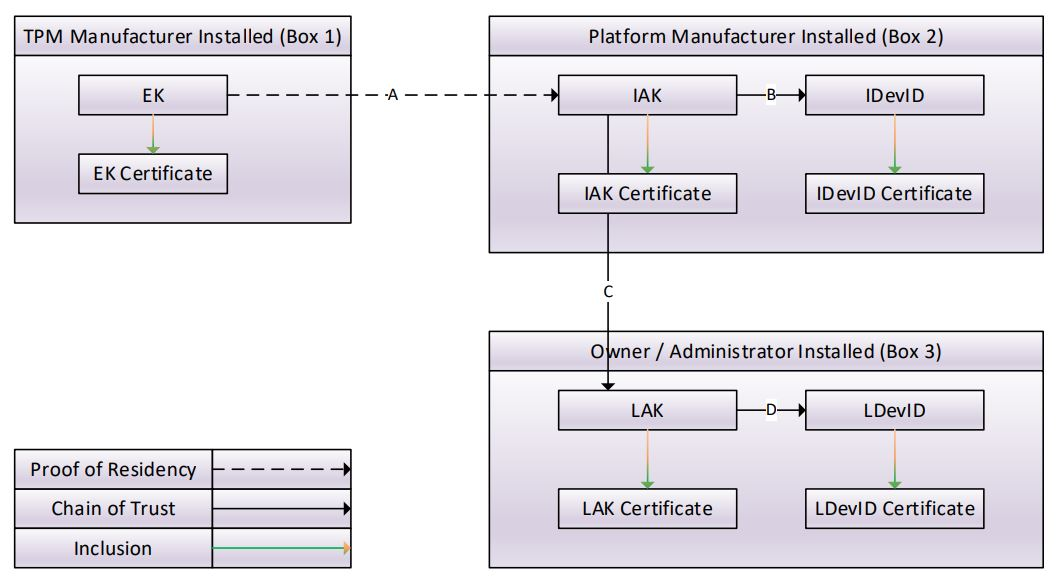
\includegraphics[width=\linewidth]{chap_3_figures/certificateRelationships.jpg}
  \par\end{centering}
  \caption{Key and Certificate Relationships [\cite{DevIDSpec-TCG}]}
  \label{fig:cert_rel}
\end{figure}
\begin{itemize}[itemsep=0pt,parsep=0pt,partopsep=0pt]
  \item \textsf{Box 1}: The EK certificate is signed by the TPM Manufacturer's CA and binds the EK to a specific TPM.
  \item \textsf{Line A}: The IAK is verified by the OEM's CA to have the correct key properties and to be resident in the same TPM as the EK.
  \item \textsf{Line B}: The IDevID is verified by the OEM's CA to have the correct key properties and to be resident in the same TPM as the IAK.
  \item \textsf{Box 2}: The IAK certificate and IDevID certificate is signed by the OEM's CA and binds the IAK and IDevID to a specific device.
  \item \textsf{Line C}: The LAK is verified by the Owner's CA to have the correct key properties and to be resident in the same TPM as the IAK.
  \item \textsf{Line D}: The LDevID is verified by the Owner's CA to have the correct key properties and to be resident in the same TPM as the LAK.
  \item \textsf{Box 3}: The LAK certificate and LDevID certificate is signed by the Owner's CA.
\end{itemize}

Figure \ref{fig:cert_rel} shows the relationships between keys and certificates for exactly one of each type of DevID. In practice, there often exists multiple of each type of DevID. Due to algorithm agility, an OEM usually installs multiple IAKs and IDevIDs with varying algorithms and sizes. An Owner may install new LAKs and LDevIDs as often as need. While an IDevID certificate always relies directly on an IAK certificate, an LAK or LDevID certificate may be directly reliant on either an IAK or LAK certificate. In particular, an LAK certificate may be used to enroll LDevIDs or additional LAKs creating an arbitrary long chain of certificates. All DevIDs (excluding IAKs) must be directly linked to an AK because the \verb|Restricted| attribute is necessary in proving that the new key resides in a specific TPM (i.e., the same TPM as the AK).

